% Team 38 midterm report (NeurIPS 2019 template, same as the proposal).
% Upload to Overleaf next to neurips_2019.sty, with the figures training_curves.png (docs/baseline/) and
% gaps_tcn.png (docs/stress_test/).
%
% Rubric (midterm column) -> section:
%   Abstract ............................ abstract
%   Motivation & objectives ............. Sec 1
%   Literature review, background ....... Sec 2
%   Model description (table) ........... Sec 3.1, Table 1
%   Dataset (prep, batch sampling) ...... Sec 3.2 (split sizes in Table 3)
%   Evaluation metric ................... Sec 3.3
%   Loss function ....................... Sec 3.4
%   Experimental depth .................. Sec 4 (2 TCNs x 13 splits x 3 seeds, LSTMs, controls, Liu)
%   Baseline (MANDATORY) + reproduction . Sec 4.1, Table 2, Fig 1
%   Implemented extensions .............. Sec 4.2 (stress test, wind split)
%   Results (preliminary) ............... Sec 5, Table 3, Fig 2
%   Discussion (challenges, risks) ...... Sec 6
%   Future directions (2-3 actions) ..... Sec 7
%   Bibliography, contributions, GitHub . end

\documentclass{article}

% Numeric citations ([1], [2], ...) as suggested by the template
\PassOptionsToPackage{numbers, compress}{natbib}

\usepackage[final]{neurips_2019}
\usepackage[utf8]{inputenc}
\usepackage[T1]{fontenc}
\usepackage{hyperref}
\usepackage{url}
\usepackage{booktabs}
\usepackage{amsmath}
\usepackage{amsfonts}
\usepackage{nicefrac}
\usepackage{microtype}
\usepackage{graphicx}
\graphicspath{{figures/}{../../docs/baseline/}{../../docs/stress_test/}}

\title{Team 38 Midterm Report\\Beyond the Training Grid: Generalization and Uncertainty in Deep Energy Models for Delivery Drones}

\author{
  Aaryan Desai \\ MRSD, Robotics Institute \\ Carnegie Mellon University \\ \texttt{aaryand@andrew.cmu.edu} \And
  Bill Ouyang \\ MRSD, Robotics Institute \\ Carnegie Mellon University \\ \texttt{blouyang@andrew.cmu.edu} \AND
  Ashutosh Kumar \\ MRSD, Robotics Institute \\ Carnegie Mellon University \\ \texttt{ashutosk@andrew.cmu.edu} \And
  Yashasvi Sorapalli \\ MRSD, Robotics Institute \\ Carnegie Mellon University \\ \texttt{ysorapal@andrew.cmu.edu}
}

\begin{document}
\maketitle

\begin{abstract}
Delivery operators must predict a drone's energy use before takeoff. Choudhry et al.~\cite{choudhry2021} showed
that a temporal convolutional network (TCN) trained on flight logs predicts quadrotor power better than a physics
model, but tested it only on payload, speed and altitude levels seen in training. We ported their models to
PyTorch, reproduced their results, and stress-tested them on held-out conditions against size-matched controls,
scoring both only on flights neither saw. Holding out a payload, speed range or altitude raises the small TCN's
power error by at most 0.4 percentage points (7--10\% MAPE), and both TCNs beat the Liu physics model (11--14\%)
everywhere. On a new route and on a wind split we built from the raw anemometer and GNSS logs, both TCNs lose about
one point. Retrained LSTMs are unreliable: 16 of 30 runs collapse to a constant, which we trace to dead ReLU units
in the output head.
\end{abstract}

\section{Introduction}
A drone's power draw depends on its speed, climb rate, tilt, payload and the wind. Published energy models give
substantially different estimates even for the same drone and conditions~\cite{zhang2021}. Choudhry et
al.~\cite{choudhry2021} instead learn power directly from flight data, but split flights at random, so every test
flight reuses payload, speed and altitude levels seen in training.

\textbf{Motivation.} Operators and route planners need energy estimates they can trust before takeoff. A model
that is accurate on familiar flights but wrong on new ones gives false confidence exactly when risk is highest.

\textbf{Objectives.} As proposed, we (i) measure how the published models degrade on held-out operating conditions,
(ii) combine physics with a neural network, and (iii) add calibrated uncertainty (90\% prediction intervals with
$\approx$90\% empirical coverage). Our results (Section~\ref{sec:results}) change (ii): the TCN barely degrades on
held-out payload, speed and altitude, so the hybrid will target data efficiency and genuinely new conditions
(route, wind) instead.

\section{Related work and background}
Choudhry et al.~\cite{choudhry2021} predict power at each time step from a 20-step window of airspeed, its
components, vertical speed and angle of attack, plus air density and payload. Their best TCN reaches 9.06\% test
MAPE versus 12.70\% for the Liu physics model~\cite{liu2017}, and they score Monte Carlo energy distributions with
Conditional Value-at-Risk (CVaR). We use their code~\cite{cvarcode}, metrics and baselines, so our numbers are
directly comparable. Liu et al.~\cite{liu2017} model power as induced, profile and parasitic terms with five fitted
constants; Zhang et al.~\cite{zhang2021} show that such physics models disagree widely. Rodrigues et
al.~\cite{rodrigues2021} released the flight logs (DJI Matrice 100, Penn Hills, PA). For uncertainty we draw on
deep ensembles~\cite{lakshminarayanan2017} and Monte Carlo dropout~\cite{gal2016}.

\section{Methods}
\subsection{Models}
All networks map a window $x_{t-19:t}\in\mathbb{R}^{20\times5}$ of time-varying inputs (airspeed $x$/$y$
components, vertical speed, angle of attack, airspeed) and two static inputs (air density, payload) to the power
$\hat y_t$ at the last step (Table~\ref{tab:models}). The TCN backbone is a stack of residual blocks of two causal
dilated convolutions (kernel 2, dilations 1--16, ReLU), and its last-step features are concatenated with the
static inputs. The LSTM backbone has three stacked layers and carries its state across a flight (stateful,
batch size 1). Both feed a head of Linear$\to$ReLU$\to$Linear (10 hidden units).

\begin{table}[ht]
\centering
\caption{Models. Inputs: window $[B,20,5]$ + static $[B,2]$; output: power $[B,1]$. PyTorch LSTMs have two
bias vectors per gate (Keras: one), hence 768 / 192 more parameters than in~\cite{choudhry2021}.}
\label{tab:models}
\small
\begin{tabular}{lllr}
\toprule
Model & Backbone (per-step feature map) & Head input & Parameters \\
\midrule
Liu physics model~\cite{liu2017} & closed form, 5 fitted constants & -- & 5 \\
s-TCN & 5 residual blocks, 16 filters: $[B,20,16]$ & 16 + 2 & 5,225 \\
b-TCN & 5 residual blocks, 64 filters: $[B,20,64]$ & 64 + 2 & 76,073 \\
s-LSTM & 3 layers, 16 units: $[B,20,16]$ & 16 + 2 & 6,025 \\
b-LSTM & 3 layers, 64 units: $[B,20,64]$ & 64 + 2 & 85,417 \\
\bottomrule
\end{tabular}
\end{table}

\subsection{Dataset and splits}
We use the authors' preprocessed flights~\cite{cvarcode}: 187 flights of a DJI Matrice 100 at 5\,Hz, 179 on the
main triangular route covering every combination of payload (0/250/500\,g), speed (4--12\,m/s) and altitude
(25--100\,m), and 8 on other routes.\footnote{Our proposal quoted 195 + 10 flights from the full dataset
release; 187 of them have preprocessed data. We take route labels from the release's
\texttt{parameters.csv}~\cite{rodrigues2021}, which corrects two flights that the authors' flight sheet mislabels.}
The target is battery voltage $\times$ current. Inputs are min--max normalized with statistics from the training
and validation flights (payload and density are left raw), and training samples batches of 32 overlapping 20-step
windows from training flights only (TCN; the stateful LSTMs use batch size 1).

Besides the paper's random split (114/38/35 train/val/test flights), each held-out split tests on every
main-route flight with one condition: 500\,g (\texttt{payload500}, extrapolation), 250\,g (\texttt{payload250},
interpolation), 12, 10--12 or 8--12\,m/s (\texttt{speed12}, \texttt{speed10-12}, \texttt{speed8-12}), 100\,m
(\texttt{alt100}) or cruise wind above 4.34\,m/s (\texttt{wind}); \texttt{route} tests on all off-route flights.
Validation (25\%, seed 42) is drawn from the remaining flights, so model selection never sees the held-out
condition. Training sizes are in Table~\ref{tab:gaps}.

\textbf{Wind split.} The preprocessed data has no wind, so we estimate it from the raw logs~\cite{rodrigues2021}.
In cruise, the wind is the ground velocity minus the airflow measured by the anemometer:
\begin{equation}
  \mathbf{w} = \mathbf{v}_g - s\,(\sin a, \cos a), \qquad a = \alpha + \delta ,
\end{equation}
where $\mathbf{v}_g$ is the body-frame velocity rotated by the INS heading into (east, north), $s$ and $\alpha$
are the anemometer speed and the compass direction the air comes from, and $\delta=-9.4^\circ$ is the 2019
magnetic declination at the site (WMM2015). These conventions make the wind consistent between the legs of the
route; the alternative readings of the angle disagree 4--7$\times$ more. A flight's wind is its cruise mean, and
\texttt{wind} holds out the windiest 20\% of main-route flights.

\subsection{Evaluation}
Following~\cite{choudhry2021}, the power error of flight $i$ with $T_i$ scored steps, measured power $y_t$ and
prediction $\hat y_t$, and its energy error over the flight's regimes $r$ (take-off, cruise, turns, landing,
found by change-point detection on pitch) are
\begin{equation}
  \mathrm{MAPE}_i = \frac{100\%}{T_i}\sum_{t=1}^{T_i}\left|\frac{y_t-\hat y_t}{y_t}\right|, \qquad
  \mathrm{RE}_i = \frac{100\%}{R_i}\sum_{r=1}^{R_i}\left|\frac{E_r-\hat E_r}{E_r}\right|,
\end{equation}
where $E_r$ is the Simpson-integrated energy of regime $r$. Both are averaged over flights, skipping each flight's
first 19 steps (no full window). Two controls make the stress test fair. (1) \textbf{Size-matched control}: for
each held-out split, a model trained on a random subset of the random split's training flights of the same size,
which isolates the unseen condition from having less data. The random split trains on most windy flights, so the
\texttt{wind} control instead tests on a random half of them and may train on the other half. (2) \textbf{Unseen flights only}: both models are scored on the $n$ held-out flights
that \emph{neither} trained or validated on (Table~\ref{tab:gaps}). We report
\begin{equation}
  \mathrm{gap} = \overline{\mathrm{MAPE}}_{\text{held-out}} - \overline{\mathrm{MAPE}}_{\text{control}},
\end{equation}
averaged over 3 seeds (mean $\pm$ std over seeds).

\subsection{Loss and optimization}
All networks minimize the mean squared error of normalized power. TCNs use Adam (learning rate $10^{-3}$,
$\epsilon=10^{-7}$, batch size 32); LSTMs use RMSprop (learning rate $10^{-3}$, $\rho=0.9$, batch size
1).\footnote{Our proposal stated a learning rate of 0.002. The released code passes the optimizer by name, so Keras
uses its default of $10^{-3}$; our port matches the released code.} We train for 30 epochs (the authors used 100;
30 already matches them for the TCNs and the s-LSTM, Table~\ref{tab:repro}) and evaluate the final epoch.

\section{Experiments}
\subsection{Baseline reproduction}
Bill ported the authors' Keras TCN and LSTM~\cite{cvarcode} to PyTorch and converted their checkpoints (output
difference $<4\cdot10^{-7}$). The converted models reproduce the paper's power MAPE to within 0.01 points
(Table~\ref{tab:repro}). The energy error matches for Liu and the LSTMs and is 0.2--0.4 points higher for the
TCNs, as it also is with the authors' own TensorFlow code, so we attribute it to library versions rather than the
port. Retrained from scratch, both TCNs match the paper over 3 seeds (s-TCN 8.86$\pm$0.26\% vs 9.13\%, b-TCN
8.92$\pm$0.16\% vs 9.06\% test MAPE), as does the s-LSTM (12.42\% vs 12.36\%, one seed). The b-LSTM does not
(16.80\% vs 11.47\%; Section~\ref{sec:discussion}). Fig.~\ref{fig:baseline} shows training curves.

\begin{table}[t]
\centering
\caption{Reproduction: power MAPE / energy RE (\%) on the paper's flight sets (``Random'': 10 fixed flights, mostly
off-route; ``Test'': 37-entry list). Top: authors' checkpoints converted to PyTorch; bottom: retrained from scratch.}
\label{tab:repro}
\small
\begin{tabular}{lcccc}
\toprule
& \multicolumn{2}{c}{Paper~\cite{choudhry2021}} & \multicolumn{2}{c}{Ours (PyTorch)} \\
Model & Random & Test & Random & Test \\
\midrule
Liu & 14.05 / 9.16 & 12.70 / 7.41 & 14.05 / 9.10 & 12.70 / 7.36 \\
b-LSTM & 13.58 / 10.35 & 11.47 / 7.57 & 13.58 / 10.37 & 11.47 / 7.59 \\
s-LSTM & 15.35 / 11.65 & 12.36 / 8.24 & 15.34 / 11.61 & 12.36 / 8.23 \\
b-TCN & 10.38 / 7.38 & 9.06 / 5.12 & 10.38 / 7.82 & 9.06 / 5.37 \\
s-TCN & 10.36 / 7.56 & 9.13 / 5.52 & 10.36 / 7.99 & 9.13 / 5.75 \\
\midrule
\multicolumn{5}{l}{\emph{Retrained from scratch, 30 epochs}} \\
b-TCN (3 seeds) & -- & -- & 9.82$\pm$0.43 / 6.74$\pm$0.68 & 8.92$\pm$0.16 / 4.98$\pm$0.19 \\
s-TCN (3 seeds) & -- & -- & 9.74$\pm$0.59 / 6.38$\pm$0.71 & 8.86$\pm$0.26 / 4.85$\pm$0.28 \\
b-LSTM (seed 0) & -- & -- & 16.29 / 11.97 & 16.80 / 12.97 \\
s-LSTM (seed 0) & -- & -- & 12.66 / 7.32 & 12.42 / 7.44 \\
\bottomrule
\end{tabular}
\end{table}

\begin{figure}[t]
\centering
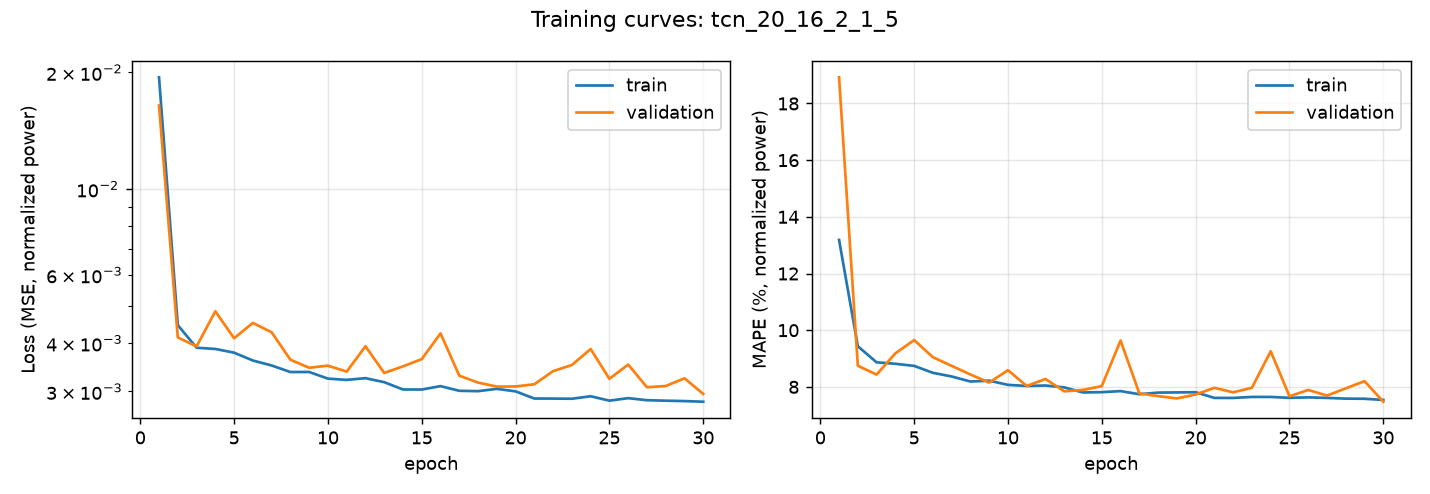
\includegraphics[width=0.6\linewidth]{training_curves.png}
\caption{Retrained s-TCN (seed 0): training and validation loss and MAPE (on normalized power) per epoch; no
overfitting.}
\label{fig:baseline}
\end{figure}

\subsection{Stress test}
Both TCNs ran every held-out split and its control with 3 seeds (78 runs); the LSTMs ran \texttt{wind} and its
control with 3 seeds and the other splits with one (b-LSTM all eleven, s-LSTM seven). The nested speed splits were
added after \texttt{speed12} showed no gap. Liu is scored on the same flights.

\section{Results}\label{sec:results}
\begin{table}[t]
\centering
\caption{Stress test (3 seeds). Train: training flights; $n$: unseen held-out flights. Gap: held-out minus control
(percentage points, positive = held-out worse). Liu: MAPE on the same flights.}
\label{tab:gaps}
\small
\begin{tabular}{lrrcccc}
\toprule
& & & s-TCN MAPE & s-TCN gap & b-TCN gap & \\
Split & Train & $n$ & held-out / control & MAPE / RE & MAPE / RE & Liu \\
\midrule
\texttt{payload500} & 87 & 21 & 7.46$\pm$0.27 / 7.26$\pm$0.12 & +0.20 / +0.90 & $-$0.01 / +0.77 & 11.04 \\
\texttt{payload250} & 90 & 16 & 7.31$\pm$0.18 / 7.21$\pm$0.08 & +0.11 / +0.11 & $-$0.20 / $-$0.25 & 10.79 \\
\texttt{speed12} & 106 & 9 & 8.87$\pm$0.30 / 8.57$\pm$0.04 & +0.30 / +0.61 & +0.22 / +0.71 & 13.49 \\
\texttt{speed10-12} & 78 & 27 & 9.89$\pm$0.25 / 9.96$\pm$0.75 & $-$0.07 / $-$0.34 & +0.12 / +0.03 & 13.68 \\
\texttt{speed8-12} & 52 & 57 & 8.82$\pm$0.11 / 8.52$\pm$0.36 & +0.30 / $-$0.25 & +0.90 / $-$0.03 & 12.85 \\
\texttt{alt100} & 100 & 16 & 8.22$\pm$0.15 / 7.82$\pm$0.05 & +0.40 / +0.39 & +0.22 / +0.34 & 10.69 \\
\texttt{route} & 134 & 8 & 10.89$\pm$0.32 / 9.81$\pm$0.28 & +1.08 / +2.30 & +1.30 / +2.71 & 13.67 \\
\texttt{wind} & 107 & 20 & 11.55$\pm$0.21 / 10.79$\pm$0.25 & +0.77 / +1.39 & +1.22 / +1.81 & 13.94 \\
\bottomrule
\end{tabular}
\end{table}

\begin{figure}[t]
\centering
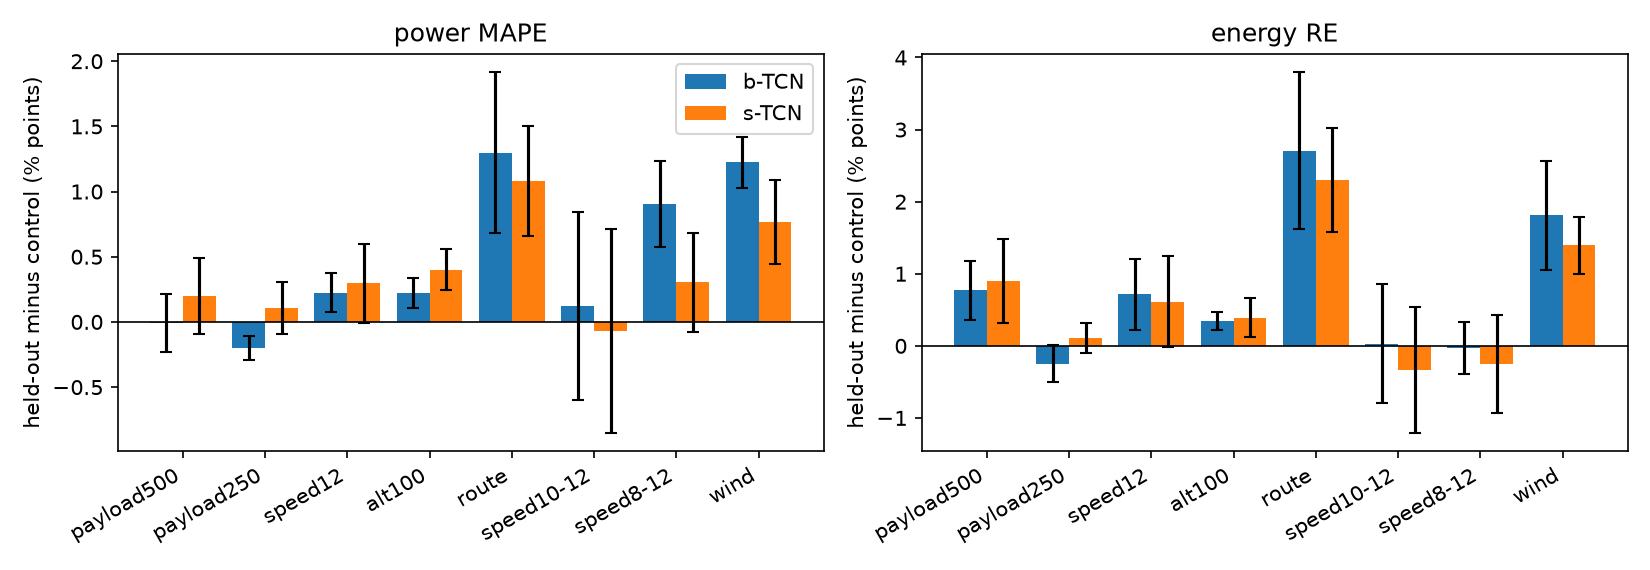
\includegraphics[width=\linewidth]{gaps_tcn.png}
\caption{Held-out minus control per split for both TCNs, in power MAPE (left) and energy RE (right). Error bars
combine the seed std of both models.}
\label{fig:gaps}
\end{figure}

\textbf{Holding out a grid condition barely hurts the TCNs} (Table~\ref{tab:gaps}, Fig.~\ref{fig:gaps}). For the
s-TCN it costs at most 0.4 MAPE points, about the spread between seeds; only \texttt{alt100} is consistent across
seeds, and extrapolating to 500\,g costs barely more than interpolating to 250\,g. The b-TCN (15$\times$ the
parameters) stays within $\pm$0.3 points except \texttt{speed8-12} (+0.90 MAPE, but $-$0.03 RE). Both TCNs beat
Liu on every split, by 2.0--4.6 points. We report no LSTM gaps, because most retrained LSTMs collapsed
(Section~\ref{sec:discussion}).

\textbf{Speed is not an extrapolation in this dataset} (failure analysis). We expected the largest gap on speed,
since parasitic power grows with airspeed, yet even \texttt{speed8-12} (trained on 4--6\,m/s) shows none for the
s-TCN. Mean flight power is nearly flat across commanded speeds (521--535\,W), because take-off, climb, hover and
landing dominate, and the \emph{measured} airspeed the network sees includes wind: 4--6\,m/s training flights
already reach 14.1\,m/s, versus 18.1\,m/s on test.

\textbf{New route.} \texttt{route} has the largest gap (+1.08 MAPE, +2.30 RE), but it is not a clean
comparison: all off-route flights are in the random split's test set, so the control has never seen them either.

\textbf{Wind is a real shift.} Unlike \texttt{route}'s, the \texttt{wind} control has seen windy flights (12 in
training), yet both TCNs are worse on unseen windy flights by +0.77$\pm$0.33 (s-TCN) and +1.22$\pm$0.20 (b-TCN)
MAPE points (+1.4 / +1.8 RE), 2--6 times the seed spread. Caveat: wind clusters by date (half of the 36 windy
flights are from two days), so it is partly a date split.

\textbf{Ablation (training-set size).} The controls share the random split's test flights, so they show what less
data costs: test MAPE is 8.86$\pm$0.26 with 114 training flights, 8.64$\pm$0.13 with 87, 10.33$\pm$0.86 with 78
and 8.88$\pm$0.21 with 52. Halving the data costs nothing on average, but the 78-flight subset is the worst on
every seed: \emph{which} flights are used matters more than how many.

\section{Discussion}\label{sec:discussion}
\textbf{Significance.} The published TCN generalizes across the payload, speed and altitude grid far better than
we expected; a planner can trust it on unseen grid points, but not yet on new routes or in wind.
\textbf{Methodology matters.} Without size-matched controls and unseen-flight scoring, the ``gap'' would mix the
condition shift, less training data and training error. \textbf{Challenges and limitations.} (i) Some comparisons
rest on 8--21 flights, and the seed spread is as large as most gaps. (ii) The grid is coarse, and a held-out speed
is still bracketed by measured airspeed. (iii) The wind estimate is noisy ($\approx$4.5\,m/s between
legs), so it separates windy from calm days rather than ranking flights. (iv) The authors fit Liu's
constants on all flights, which slightly favors Liu. (v) \textbf{Retrained LSTMs collapse.} 16 of our 30 LSTM runs
predict a constant: all 10 ReLU units of the output head are inactive on every input, so the output is the last
bias and no gradient reaches the LSTM. Survivors keep 1--4 active units, hence 3--6 point validation swings. We
attribute this to batch-size-1 RMSprop (90k learning-rate-sized steps per epoch vs 2.8k averaged Adam steps for the
TCN); our port matches the Keras defaults and the authors' script saves only periodic snapshots, so we cannot tell
whether their runs were affected. \textbf{Risk.} A hybrid may not beat a TCN that already generalizes.

\section{Next steps}
\begin{enumerate}
\item \textbf{Physics + TCN hybrid} $\hat y_t = P_{\mathrm{Liu}}(x_t) + g_\theta(x_{t-19:t})$, with Liu's constants
refit per split, evaluated as a learning curve (5--52 training flights, several subsets per size) and on
\texttt{route}/\texttt{wind}.
\item \textbf{Uncertainty:} a Gaussian variance head (NLL loss), a deep ensemble (our 3 seeds) and MC dropout; 90\%
interval coverage on the held-out splits, then the authors' CVaR pipeline.
\item \textbf{LSTMs and completeness:} fix LSTM training (leaky ReLU head, lower learning rate or Adam), run both
LSTMs on every split with 3 seeds, add a date-matched \texttt{wind} control; defer the proposed transformer.
\end{enumerate}

\section*{Team contributions and code}
Code: \url{https://github.com/wouyang26/idl_project_38}.
\textbf{Bill Ouyang}: PyTorch port and checkpoint conversion, reproduction of the paper's results, b-TCN
stress-test runs.
\textbf{Yashasvi Sorapalli}: 30-epoch s-TCN baseline and figures, first held-out splits, b-LSTM stress-test runs.
\textbf{Ashutosh Kumar}: s-LSTM experiments and stress-test runs, evaluation fixes.
\textbf{Aaryan Desai}: data pipeline, Liu evaluation, size-matched controls and unseen-flight scoring, nested speed
splits, stress-test pipeline, s-TCN runs, wind split and its runs, LSTM collapse diagnosis.

\small
\begin{thebibliography}{9}

\bibitem{choudhry2021}
A.~Choudhry, B.~Moon, J.~Patrikar, C.~Samaras, and S.~Scherer.
\newblock CVaR-based flight energy risk assessment for multirotor UAVs using a deep energy model.
\newblock In {\it IEEE International Conference on Robotics and Automation (ICRA)}, pp.\ 262--268, 2021.

\bibitem{cvarcode}
A.~Choudhry, B.~Moon, and J.~Patrikar.
\newblock cvar-energy-risk-deep-model (code and pretrained models).
\newblock \url{https://github.com/castacks/cvar-energy-risk-deep-model}, 2021.

\bibitem{rodrigues2021}
T.~A. Rodrigues, J.~Patrikar, A.~Choudhry, et al.
\newblock In-flight positional and energy use data set of a DJI Matrice 100 quadcopter for small package delivery.
\newblock {\it Scientific Data}, 8, 2021. Data: \url{https://doi.org/10.1184/R1/12683453}.

\bibitem{liu2017}
Z.~Liu, R.~Sengupta, and A.~Kurzhanskiy.
\newblock A power consumption model for multi-rotor small unmanned aircraft systems.
\newblock In {\it International Conference on Unmanned Aircraft Systems (ICUAS)}, pp.\ 310--315, 2017.

\bibitem{zhang2021}
J.~Zhang, J.~F. Campbell, D.~C. Sweeney II, and A.~C. Hupman.
\newblock Energy consumption models for delivery drones: A comparison and assessment.
\newblock {\it Transportation Research Part D}, 90:102668, 2021.

\bibitem{lakshminarayanan2017}
B.~Lakshminarayanan, A.~Pritzel, and C.~Blundell.
\newblock Simple and scalable predictive uncertainty estimation using deep ensembles.
\newblock In {\it Advances in Neural Information Processing Systems 30}, 2017.

\bibitem{gal2016}
Y.~Gal and Z.~Ghahramani.
\newblock Dropout as a Bayesian approximation: Representing model uncertainty in deep learning.
\newblock In {\it International Conference on Machine Learning (ICML)}, 2016.

\end{thebibliography}

\end{document}
